\section{Langkah-Langkah Percobaan}

\subsection{Percobaan Crimping}
\begin{enumerate}
	\item Kabel LAN dikuliti sepanjang seutas jari dengan alat pemotong
	\item Urutkan kabel sesuai dengan urutan warna kabel
	\item Setelah itu crimping dengan konektor menggunakan alat crimping
	\item Test kabel LAN yang sudah dicrimping dengan  alat tester untuk mengetahui kabel crimping sudah benar atau belum
\end{enumerate}

\subsection{Percobaan Routing Statis}
\begin{enumerate}
    \item Masuk ke Winbox untuk mereset router
    \item Lalu hubungkan router ke PC menggunakan kabel LAN, dan login ke router dengan MAC address
    atau iP address default
    \item Lalu konfigurasi IP address pada sambungan ether 1 untuk digunakan sebagai jalur antar router pada kedua laptop
    \item Lalu konfigurasi IP address pada sambungan ether 2 untuk digunakan sebagai jalur ke PC pada kedua laptop
    \item Selanjutnya menambahkan IP address dengan manual. Masuk ke meu IP, lalu pilih routes, Untuk router 1 
    gunakan alamat network router 2, dan untuk router 2 gunakan alamat network router 1,dan untuk 
    ether gateway 1 gunakan alamat ether 2, dan untuk ether gateway 2 gunakan alamat ether 1.
    \item Lalu konfigurasikan IP address pada laptop dengan cara manual interface menggunakan setting
    windows, dengan router 1 dan router 2 konfigurasikan IP,netmask,dan gateway sesuai dengan tujuan
    \item Lalu uji ping untuk mengetest konektivitas antara laptop 1 dan laptop 2  
\end{enumerate}


\subsection{Percobaan Routing Dinamis}
Pada percobaan ini kosong karena kelompok kami belum berhasil melakukan percobaan routing statis,
sehingga kami tidak bisa melanjutkan ke Routing Dinamis.

\section{Analisis Hasil Percobaan}
Kabel LAN memiliki sebuah urutan yang perlu diikuti untuk pengkonfigurasi kabelnya, saat terdapat kesalahan
mengurutkan kabel yang sudah dikuliti dan dipasang dengan konektor, maka saat ditest menggunakan alat 
pengecekan, pada alat lampu yang berkedip tidak sesuai dengan urutan yang sudah ditentukan oleh alat tersebut.
Pada percobaan routing statis, kami tidak berhasil melakukan percobaan, kami mungkin ada kesalahan pada penginputan 
alamat IP address, baik itu pada alamat IP untuk router 1 dan router 2, atau juga alamat untuk menghubungkan
laptop dengan router. Pada percobaan routing dinamis, kami tidak bisa melanjutkan percobaan ini karena kami belum berhasil
melakukan percobaan routing statis, sehingga kami tidak bisa melanjutkan ke routing dinamis, dan waktunya
sudah habis
\section{Hasil Tugas Modul}
\begin{enumerate}
    \item Terdapat 4 subnet, di mana masing masing subnet akan diisi oleh 4 departemen, dan terdapat 1 switch
    yang berfungsi sebagai penghubung antar semua device yang ada pada subnet ke Router,di setiap PC dan switch
    sudah dikongifurasikan untuk alamat IP dan gateway. 
	\begin{figure}[H]
		\centering
		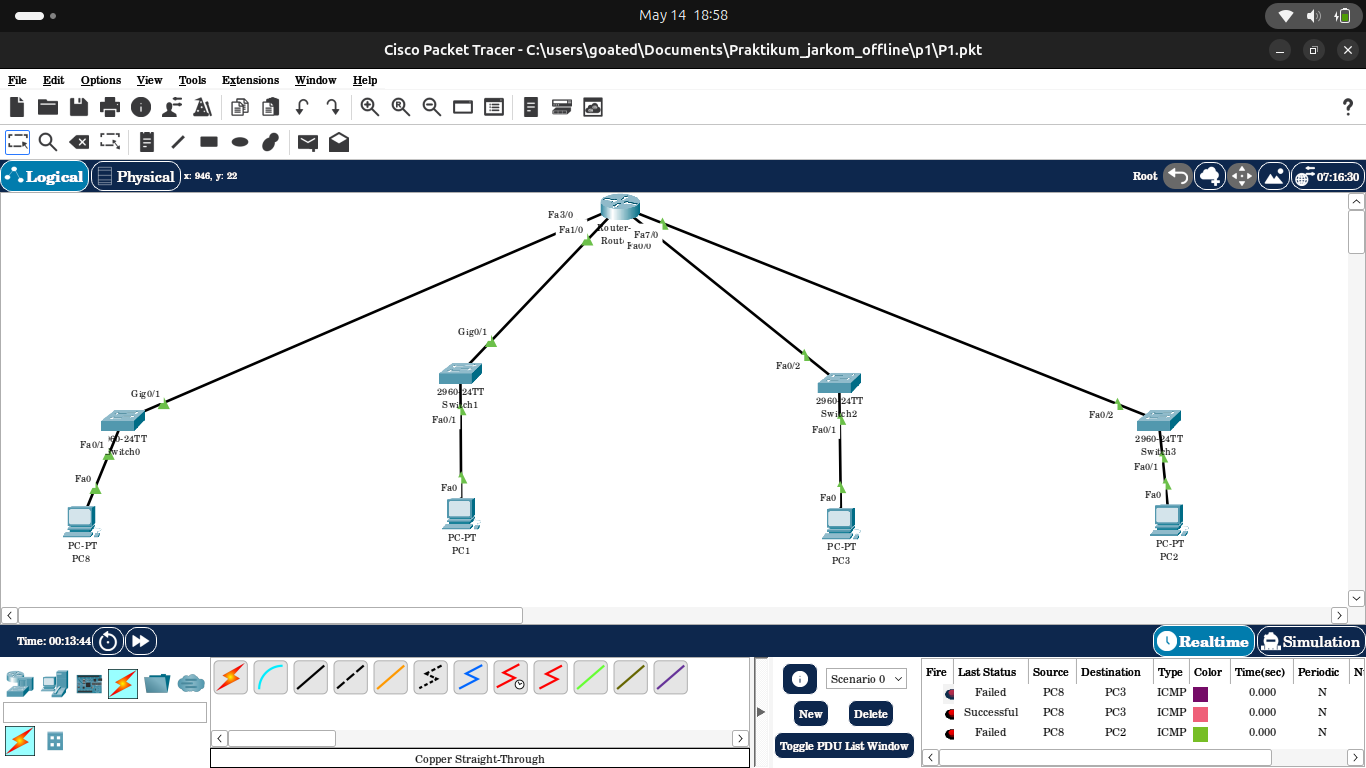
\includegraphics[width=0.5\linewidth]{cisco.png}
		\caption{Gambar Topologi pada Cisco Packet Tracer}
		\label{fig:gambar1}
	\end{figure}
\end{enumerate}


\section{Kesimpulan}
Dari percobaan yang sudah dilakukan,dapat disimpulkan bahwa kabel LAN memiliki urutan kabel yang harus diikuti,sehingga
kabel LAN dapat berfungsi dengan baik, dan saat dilakukan pengujian menggunakan alat tester, lampu yang berkedip.
Pada percobaan routing statis, kami tidak berhasil melakukan percobaan ini, kami mungkin ada kesalahan pada penginputan
atau pada alat yang digunakan baik itu software atau hardware, sehingga kami tidak bisa melanjutkan ke routing dinamis. Pada percobaan routing dinamis,

\section{Lampiran}
\subsection{Dokumentasi saat praktikum}
	\begin{figure}[H]
		\centering
		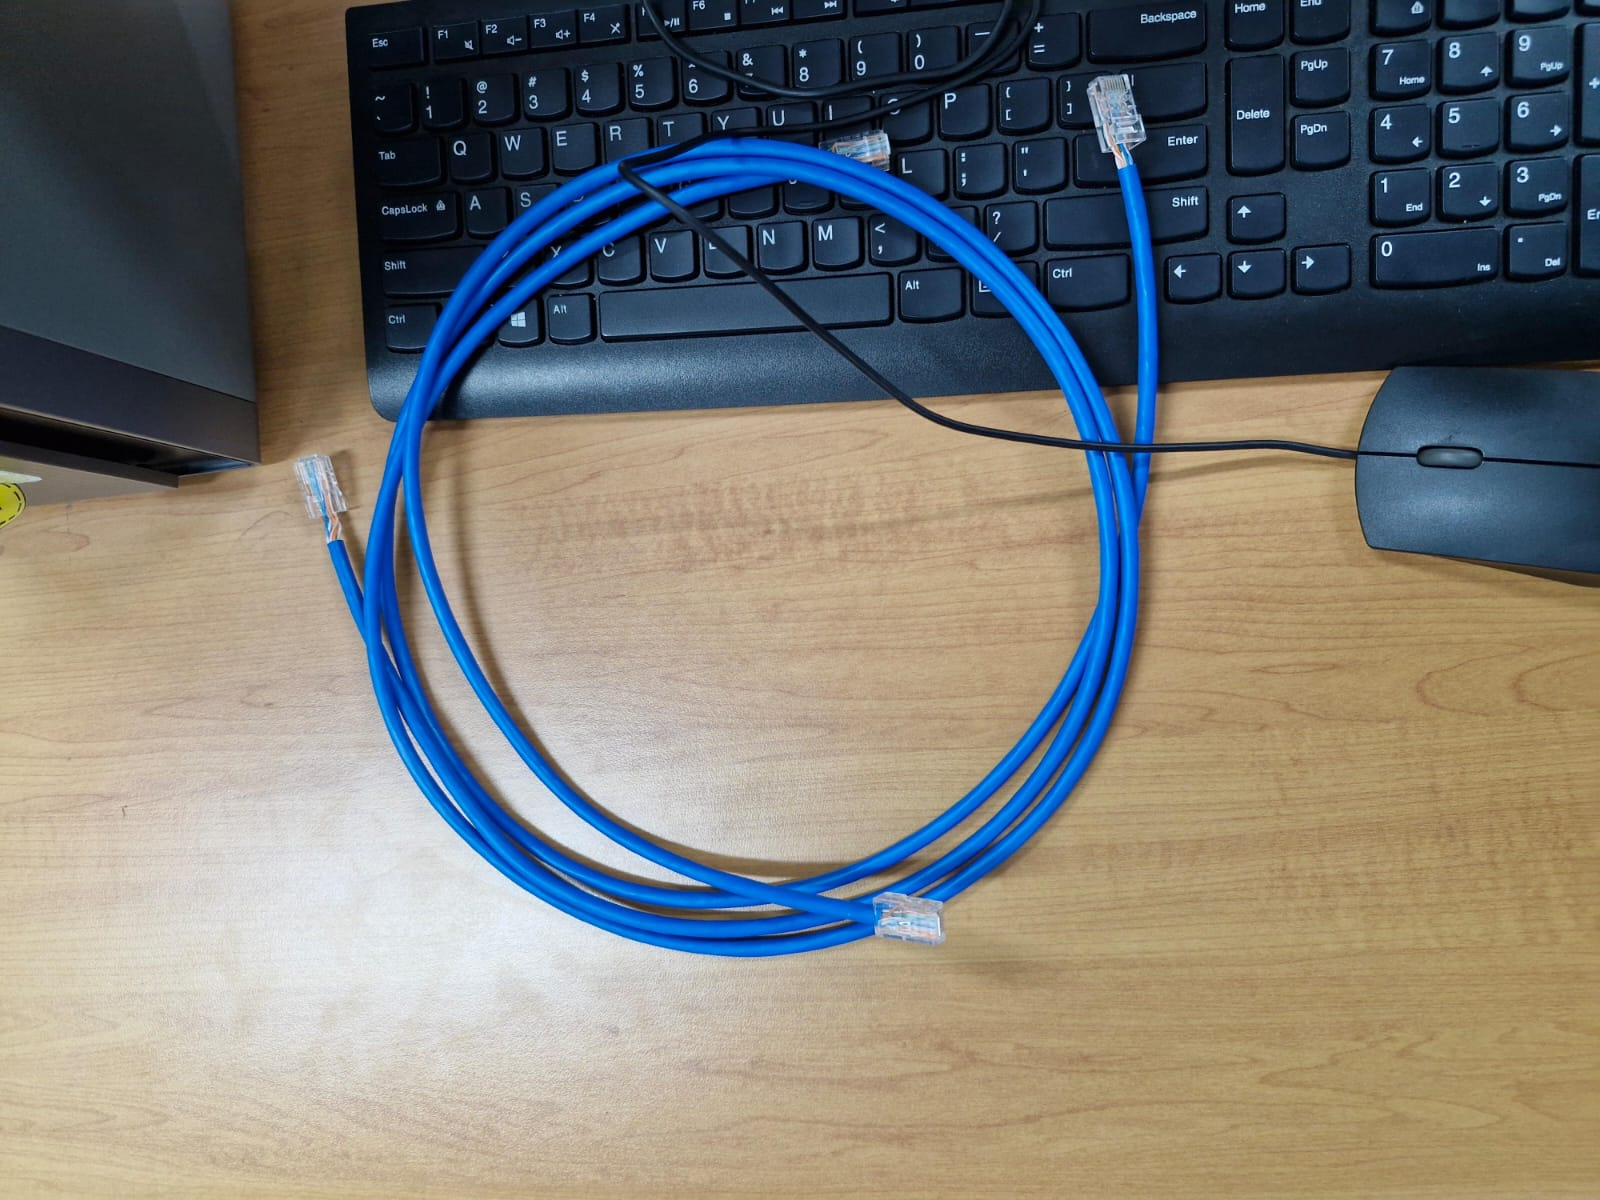
\includegraphics[width=0.5\linewidth]{1.jpeg}
		\caption{Kabel LAN Selesai di crimping}
		\label{fig:gambar1}
	\end{figure}
    	\begin{figure}[H]
		\centering
		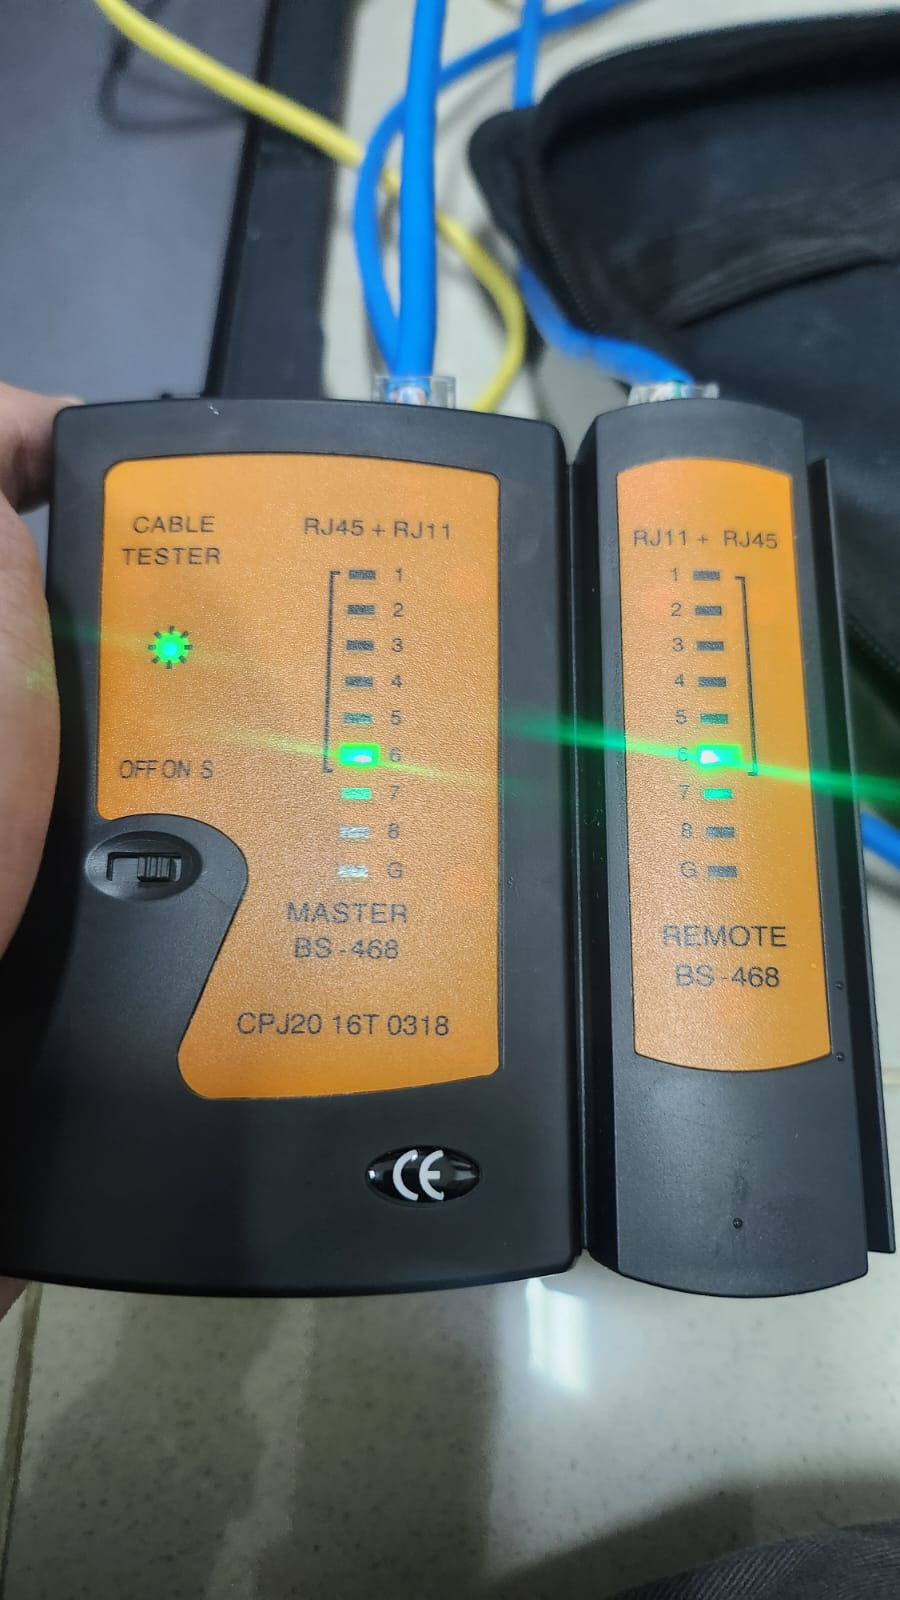
\includegraphics[width=0.5\linewidth]{2.jpeg}
		\caption{Kabel LAN Ditest}
		\label{fig:gambar1}
	\end{figure}

    \begin{figure}[H]
        \centering
        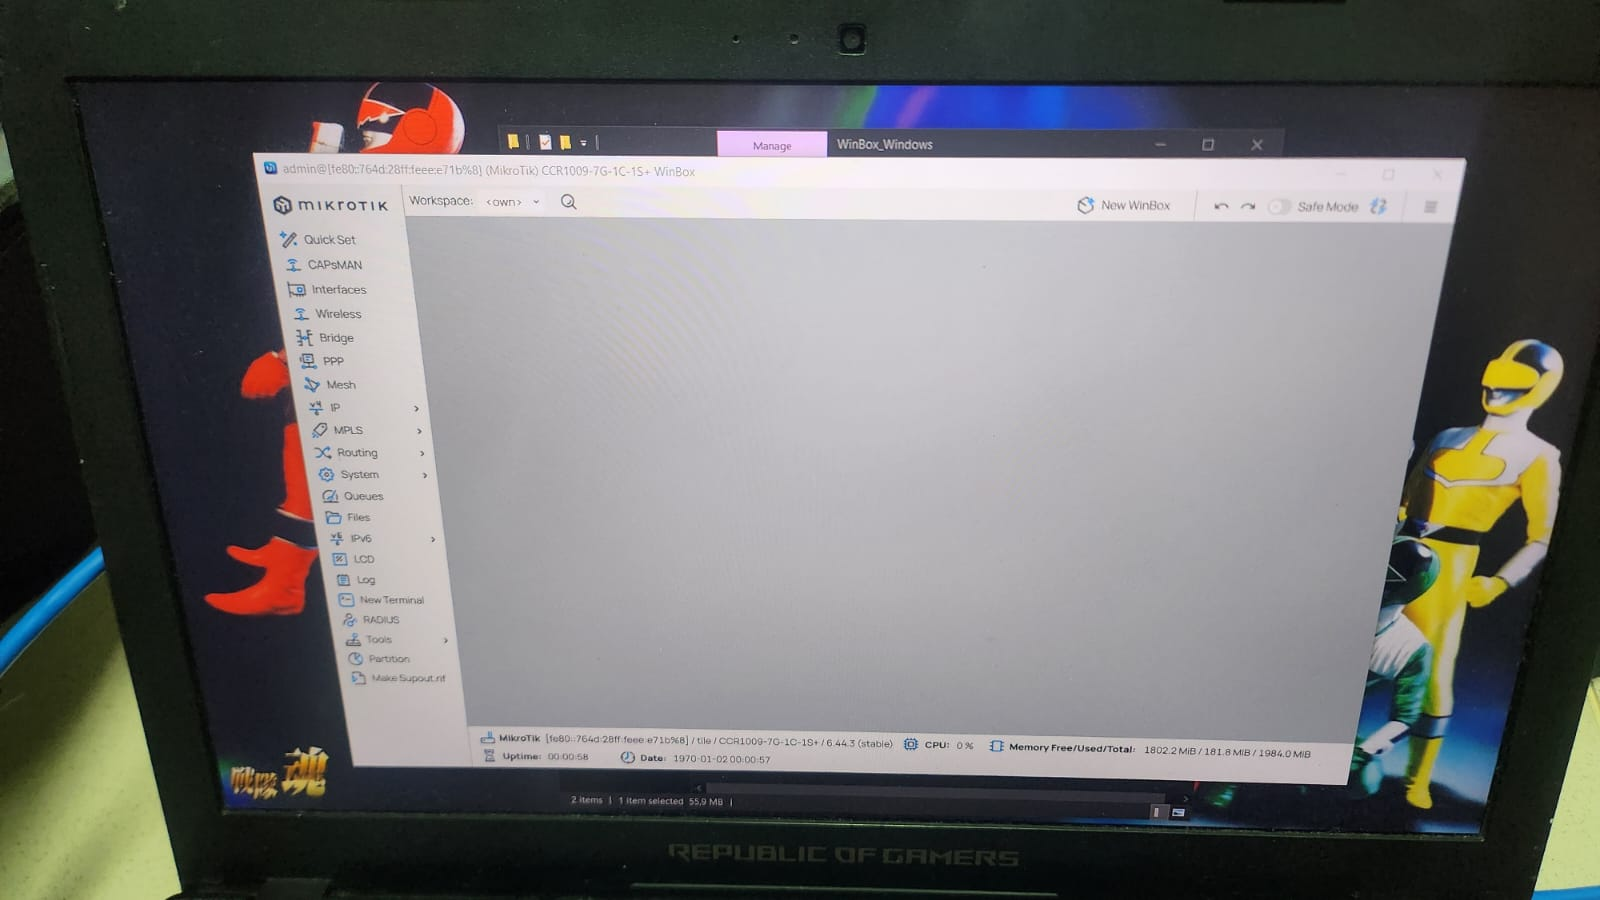
\includegraphics[width=0.5\linewidth]{3.jpeg}
        \caption{Mereset Router pada Winbox}
        \label{fig:gambar1}
    \end{figure}

    \begin{figure}[H]
        \centering
        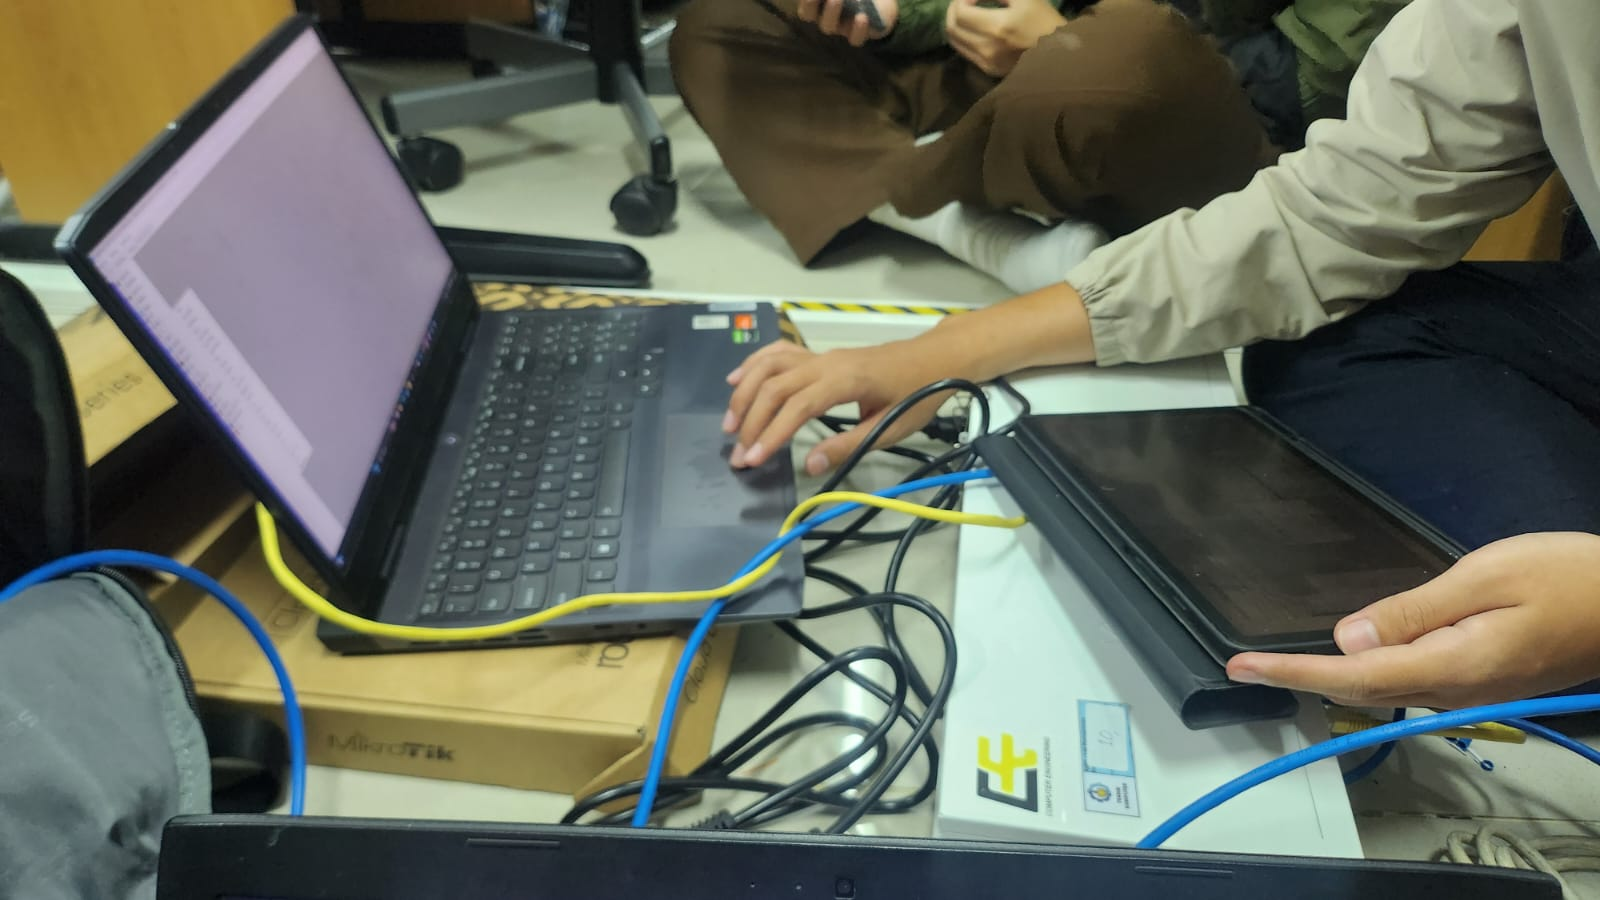
\includegraphics[width=0.5\linewidth]{4.jpeg}
        \caption{Menginput Alamat IP pada Winbox}
        \label{fig:gambar1}
    \end{figure}
    


